\documentclass[]{article}
\usepackage{lmodern}
\usepackage{amssymb,amsmath}
\usepackage{ifxetex,ifluatex}
\usepackage{fixltx2e} % provides \textsubscript
\ifnum 0\ifxetex 1\fi\ifluatex 1\fi=0 % if pdftex
  \usepackage[T1]{fontenc}
  \usepackage[utf8]{inputenc}
\else % if luatex or xelatex
  \ifxetex
    \usepackage{mathspec}
  \else
    \usepackage{fontspec}
  \fi
  \defaultfontfeatures{Ligatures=TeX,Scale=MatchLowercase}
\fi
% use upquote if available, for straight quotes in verbatim environments
\IfFileExists{upquote.sty}{\usepackage{upquote}}{}
% use microtype if available
\IfFileExists{microtype.sty}{%
\usepackage{microtype}
\UseMicrotypeSet[protrusion]{basicmath} % disable protrusion for tt fonts
}{}
\usepackage[margin=1in]{geometry}
\usepackage{hyperref}
\hypersetup{unicode=true,
            pdftitle={Microplastics in Romaine Lettuce: Lab Report},
            pdfauthor={Susannah Budd},
            pdfborder={0 0 0},
            breaklinks=true}
\urlstyle{same}  % don't use monospace font for urls
\usepackage{graphicx,grffile}
\makeatletter
\def\maxwidth{\ifdim\Gin@nat@width>\linewidth\linewidth\else\Gin@nat@width\fi}
\def\maxheight{\ifdim\Gin@nat@height>\textheight\textheight\else\Gin@nat@height\fi}
\makeatother
% Scale images if necessary, so that they will not overflow the page
% margins by default, and it is still possible to overwrite the defaults
% using explicit options in \includegraphics[width, height, ...]{}
\setkeys{Gin}{width=\maxwidth,height=\maxheight,keepaspectratio}
\IfFileExists{parskip.sty}{%
\usepackage{parskip}
}{% else
\setlength{\parindent}{0pt}
\setlength{\parskip}{6pt plus 2pt minus 1pt}
}
\setlength{\emergencystretch}{3em}  % prevent overfull lines
\providecommand{\tightlist}{%
  \setlength{\itemsep}{0pt}\setlength{\parskip}{0pt}}
\setcounter{secnumdepth}{0}
% Redefines (sub)paragraphs to behave more like sections
\ifx\paragraph\undefined\else
\let\oldparagraph\paragraph
\renewcommand{\paragraph}[1]{\oldparagraph{#1}\mbox{}}
\fi
\ifx\subparagraph\undefined\else
\let\oldsubparagraph\subparagraph
\renewcommand{\subparagraph}[1]{\oldsubparagraph{#1}\mbox{}}
\fi

%%% Use protect on footnotes to avoid problems with footnotes in titles
\let\rmarkdownfootnote\footnote%
\def\footnote{\protect\rmarkdownfootnote}

%%% Change title format to be more compact
\usepackage{titling}

% Create subtitle command for use in maketitle
\providecommand{\subtitle}[1]{
  \posttitle{
    \begin{center}\large#1\end{center}
    }
}

\setlength{\droptitle}{-2em}

  \title{Microplastics in Romaine Lettuce: Lab Report}
    \pretitle{\vspace{\droptitle}\centering\huge}
  \posttitle{\par}
    \author{Susannah Budd}
    \preauthor{\centering\large\emph}
  \postauthor{\par}
      \predate{\centering\large\emph}
  \postdate{\par}
    \date{05/04/2019}

\usepackage{booktabs}
\usepackage{longtable}
\usepackage{array}
\usepackage{multirow}
\usepackage{wrapfig}
\usepackage{float}
\usepackage{colortbl}
\usepackage{pdflscape}
\usepackage{tabu}
\usepackage{threeparttable}
\usepackage{threeparttablex}
\usepackage[normalem]{ulem}
\usepackage{makecell}
\usepackage{xcolor}

\begin{document}
\maketitle

\hypertarget{abstract}{%
\subsubsection{Abstract}\label{abstract}}

Microplastic contamination is a pressing issue, and one of particular
concern for the spheres of ecosystem and human health. Dietary
microplastic contamination has been of significant concern recently as a
potential pathway for bioaccumulation of microplastics in humans.
However, this body of literature has focused largely on the risk of
contamination through seafood, as microplastic contamination in the
ocean is particularly high. This research aimed to investigate
microplastic levels in romaine lettuce intended for human consumption
and investigate the role of plastic packaging in potential microplastic
contamination in order to gain a new perspective on dietary exposure
routes. In comparing packaged and unpackaged lettuce, the null
hypothesis of ``there is no difference in microplastic quantities in
romaine lettuce with or without plastic packaging'' could not be
rejected (p-value = 0.5839). This reality brings up further questions
concerning the extent of laboratory microplastic contamination and the
future of research into microplastics and produce.

\hypertarget{introduction}{%
\subsubsection{Introduction}\label{introduction}}

Microplastics have become a consistent component of the environment of
the entire biosphere. Plastics and their additives have been located
throughout every major body of water and in many species, including
humans (GESAMP 2016). The ubiquity of microplastics is of particular
concern as many plastic additives, such as BPA, have been shown to be
harmful to human health (Calafat et al.~2008). However, the vehicles
through which microplastics are transmitted to the human body are not
fully understood. One suspected pathway for bioaccumulation is through
foodways, however, research into the presence of microplastics in food
(other than seafood) has been limited (Karbalaei et al.~2018). This
research hopes to delve into a component of microplastics in food which
has not yet been explored - produce. Additionally, it intends to
investigate if human dependence on plastic packaging is impacting
dietary microplastic exposure, and consequently related health effects.~

Concerns surrounding the impacts of microplastics on human health have
been growing alongside scientific understanding of how plasticizers and
polymers may impact human health. A major concern surrounding both
issues has been bioaccumulation. Recently, studies have shown strong
evidence for bioaccumulation following ingestion in marine bodies from
bivalves to fin whales (Fossi et al.~2016, Batel et al.~2016).
Additionally, as was discussed by Wright and Kelly (2017), the body of
scientific literature surrounding non-plastic particle accumulation and
leaching suggests than microplastics and their associated chemicals will
be able to bioaccumulate in humans as well. Given the emerging
understanding of the potential health impacts of significant
microplastic exposure, more in-depth research regarding the scope of
foodway microplastic exposure is certainly warranted.~

One particular area of consumption which has not had significant
scientific investigation is that of produce. Due to the density of
microplastics in the ocean, investigation into microplastic
proliferation has largely centered around oceanic products, such as
seafood (Karbalaei et al.~2018). Additionally, many of these studies
focus on these products well before they are intended for human
consumption, including areas which usually aren't consumed by humans,
such as the gastrointestinal tract (Baalkhuyur et al.~2018, Rochman et
al.~2015, Karlsson et al.~2017). Because of this, there is no scientific
consensus regarding how significant dietary ingestion of microplastics
is to overall microplastic exposure. By investigating produce at the
stage of production nearest to consumption (in the grocery store), this
research aims to begin to create a more robust understanding of how all
foodways impact human microplastic exposure, and how processing tactics,
such as packaging, play a role in exposure.~

In order to begin to investigate these aims, the questions to
investigate must first be developed. For the purpose of this particular
research, the overarching questions are: Are there detectable
microplastics in romaine lettuce intended for human consumption? If yes,
do microplastic concentrations vary depending on whether or not they
were packaged in plastics? Because of romaine's availability both in
unpackaged heads and prepared plastic bags, it serves as the ideal
produce through which to investigate how the phenomenon of how packaging
impacts microplastic exposure and subsequent leaching. Furthermore, this
research will be conducted using a hypothesis test, where a null
hypothesis will be rejected or not rejected based on whether a p-value
of \textless{} 0.05 is obtained. For the purpose of this research, the
null hypothesis is ``there is no difference in microplastic quantities
in romaine lettuce with or without plastic packaging.'' This metric will
be used to assess the impact of plastic packaging on foodway
microplastic exposure.~

Most of the scientific body of research surrounding foodway paths to
microplastic exposure is focused on seafood or foods obtained many steps
before they would be presented for human consumption (Karbalaei et
al.~2018). This research aims both to focus on an area of food which has
not been previously investigated (packaged vs.~unpackaged produce), and
investigate it in a phase near human consumption so as to gain a more
thorough understanding of how significant dietary microplastic exposure
truly is. As is discussed by Rist et al. (2018), the focus on
pre-production seafood is representative of an incredibly minute amount
of microplastic exposure when compared to overall human exposure. As
they go on to note, focusing on such a relatively small issue risks
drawing attention away from the more significant and systematic issues
of plastic consumption. By drawing the attention of dietary
microplastics away from pre-production seafood, and focusing on the more
systematic issue of packaging, hopefully this research may begin to
diversity the body of scientific literature surrounding microplastics in
food.~

\hypertarget{methods}{%
\subsubsection{Methods}\label{methods}}

\begin{enumerate}
\def\labelenumi{\arabic{enumi}.}
\tightlist
\item
  Obtain Romaine lettuce. Purchase \textbf{two unpackaged heads of
  romaine lettuce} and \textbf{two heads of romaine lettuce in plastic
  packaging} (pre-chopped for salad is acceptable) from 5 nearby stores
  - Sprouts on Foothill Boulevard, Stater Bros.~on N. Garey Avenue,
  Cardenas on E. Holt Avenue, El Super on E. Holt Avenue, and Super King
  on Auto Center Drive. Upon purchasing the lettuce, ensure that it is
  carried out in \textbf{individual paper bags} to avoid contamination.
  Seal the bags to avoid contamination with airborne particulates,
  however, some contamination will likely be unavoidable.~
\item
  In the lab, obtain a \textbf{glass blender}. If unbagged, thoroughly
  wash one head of lettuce with deionized water, and then fill the
  blender with leaves until they reach the top. If bagged insert leaves
  into blender until they reach the top without washing, as the lettuce
  is labeled pre-washed.~
\item
  Add \textbf{200 mL of Milli-Q deionized water} to the blender. Blend
  for 30 seconds on the slower ``grind'' setting, then for 60 seconds on
  the faster ``cream'' setting.~
\item
  Strain the contents of each beaker through a \textbf{stainless steel
  filter with a mesh size of 5 mm} to capture larger organic fibers
  while allowing all particles meeting the qualification of
  ``microplastic'' (\textgreater{}5mm) to pass through until 100 mL of
  solution is obtained. Place this solution in a glass beaker covered
  with \textbf{aluminum foil} to avoid airborne contamination.~
\item
  Extract 5 mL of the blended lettuce solution using a \textbf{glass
  pipette} and place in a \textbf{100 mL glass beaker}. Due to the large
  quantities of cellulose in lettuce, use the enzyme cellulase from
  Niger Aspergillus niger to digest the remaining organic material while
  leaving any microplastic particles intact. Add \textbf{5 mL of
  cellulase} and \textbf{10 mL of a phosphate-buffered saline (PBS)
  solution} (1 L prepared with \textbf{8 g sodium chloride}, \textbf{200
  mg potassium chloride}, \textbf{1.44 g disodium phosphate} and
  \textbf{240 mg monopotassium phosphate in deionized water}, set to pH
  5.0 using hydrochloric acid). Cover beaker with \textbf{aluminum
  foil}.~
\item
  Incubate the solution at 50 degrees C for 4 days.~
\item
  Repeat steps 2-6 for every purchased head of lettuce.~
\item
  Add \textbf{NaCl in solution with deionized water} (density=1.2g/mL,
  stirred for 10 minutes) to the incubated solution until the beaker has
  100 mL of solution in it. Allow solution to settle for 30 minutes,
  then use a vacuum system to collect the top 40 mL of each sample and
  any floating microplastics within it.~9. Add \textbf{5 mL of 0.08 g/mL
  Nile red dye solution} to this extracted solution and wait 30 minutes
  to allow staining to occur.~
\item
  Run this extracted and stained solution through \textbf{vacuum
  filtration with an entirely glass apparatus} to separate stained
  fibers from their liquid matrix. Place the resulting filter paper in a
  \textbf{glass beaker}, cover with \textbf{aluminium foil}, and allow
  it to dry overnight.~
\item
  Use \textbf{RStudio} to generate random coordinate points. Create a
  grid on the dried filter paper, and plot four random points onto this
  grid on each paper.~
\item
  Use the \textbf{digital Revolve microscope with fluorescent light} (4x
  zoom lens, TXRED fluorescent/FL overlay at 100\% brightness, 110 ms
  capture) and use ocular techniques to count the number of fluorescent
  particles present at each marked location on the paper.~
\item
  Repeat steps 8-12 with each incubated solution.~
\item
  In order to mitigate the impacts of contamination or procedural error,
  corroborated the results through the use of \textbf{blanks}. 3 water
  ``samples'' should go through steps 2-11 alongside the experimental
  samples, but with 100 mL of deionized water rather than solution
  material. All equipment used should be washed thoroughly before and
  after touching any sample, and all water used to wash should be
  deionized so as to avoid contamination from the water.~
\item
  The methods of Loder et al.~2017, Maes et al.~2017, Wang and Wang
  2018, Karlsson et al.~2017, and Quinn et al.~2018 were consulted in
  developing these proposed procedures.
\end{enumerate}

\hypertarget{results}{%
\subsubsection{Results}\label{results}}

The data collection yielded five replicates and five pseudo-replicates
for both bagged and unbagged lettuce, as two bagged and unbagged heads
were purchased at five different stores. In order to more accurately
reflect these replicates, the number of microplastics found on each head
of lettuce was averaged with its pair. For example, the number of
microplastics found on each bagged lettuce head purchased at Cardenas
were averaged with one another. The graph below shows the box plots of
these averages for bagged and unbagged lettuce.

\begin{center}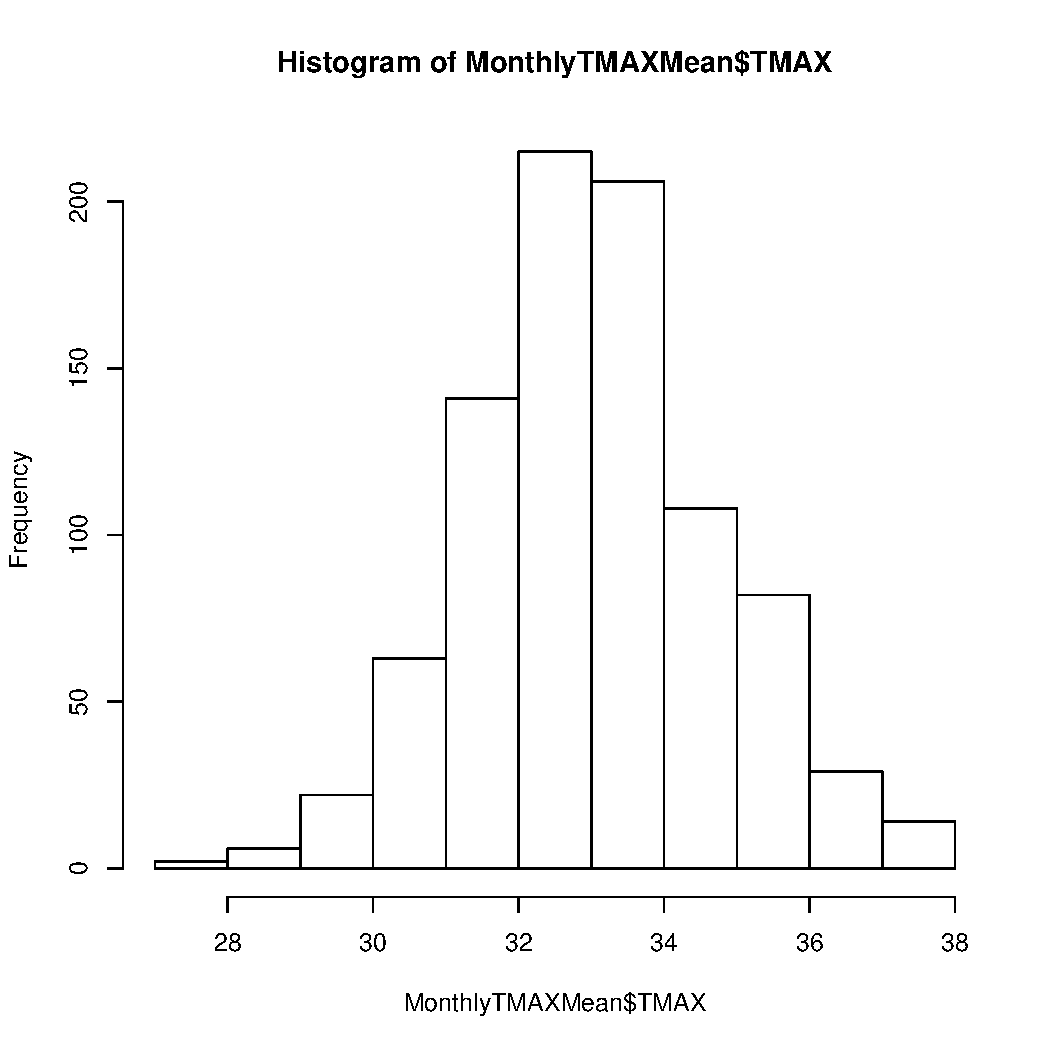
\includegraphics{Lab_Report_files/figure-latex/unnamed-chunk-2-1} \end{center}

\hypertarget{normality-tests}{%
\paragraph{\texorpdfstring{Normality Tests\\
}{Normality Tests }}\label{normality-tests}}

This experiment was designed to test the null hypothesis of ``there is
no difference in microplastic quantities in romaine lettuce with or
without plastic packaging.'' In order to determine whether or not to
reject the null hypothesis, whether or not the data fell within normal
distribution was first assessed, using Q-Q Plots and the Shapiro-Wilk
normality test.

\hypertarget{bagged}{%
\subparagraph{Bagged}\label{bagged}}

For bagged lettuce data, the Shapiro-Wilk normality test yielded a
p-value of 0.2768, indicating that it is within the bounds of normal
distribution. The Q-Q plot, shown below, also demonstrates that most
points fall within the expected bounds.

\begin{center}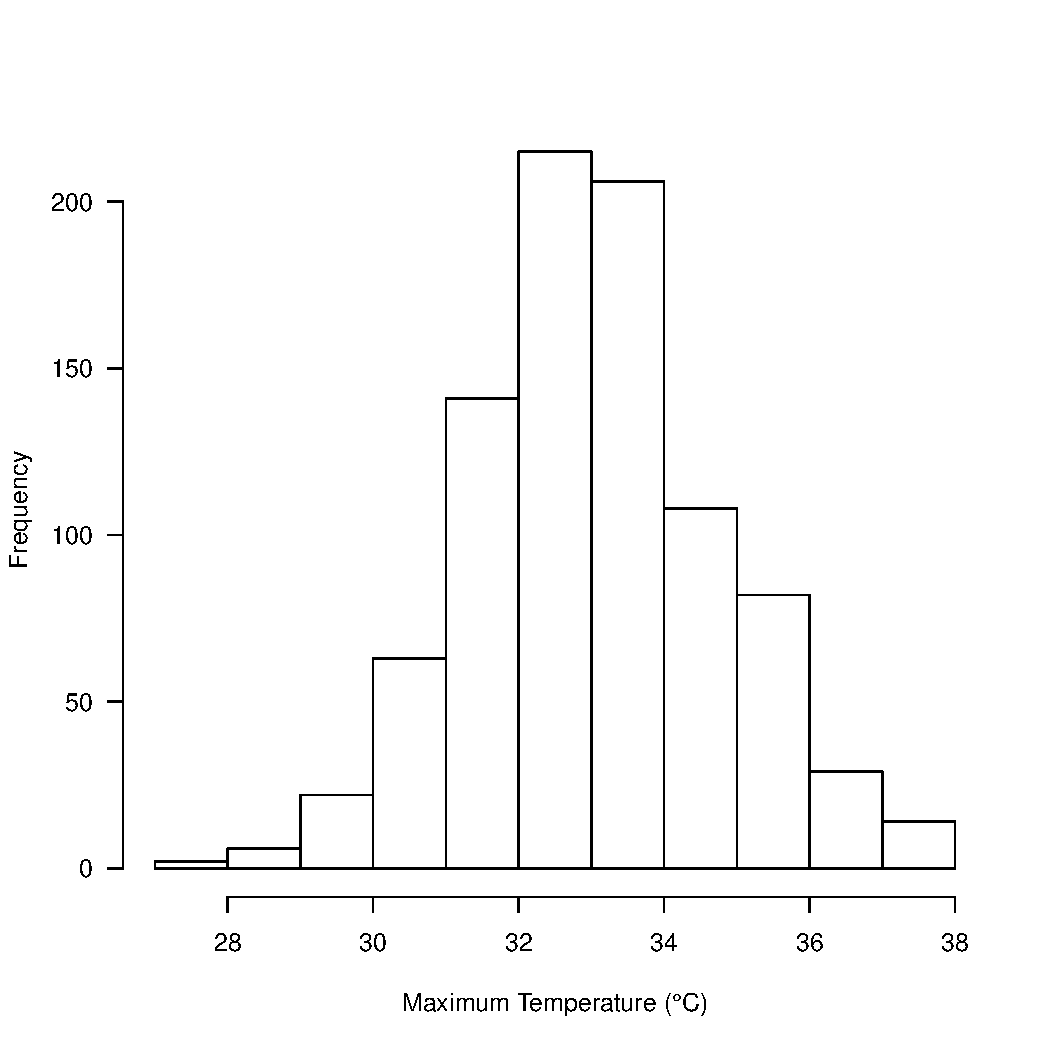
\includegraphics{Lab_Report_files/figure-latex/unnamed-chunk-3-1} \end{center}

\hypertarget{unbagged}{%
\subparagraph{Unbagged}\label{unbagged}}

For unbagged lettuce data, the Shapiro-Wilk normality test yielded a
p-value of 0.04526, indicating that it is not within the bounds of
normal distribution. The Q-Q plot, shown below, also demonstrates that,
while most points fall within the expected bounds, some are much further
out of normal distribution than they were for the bagged lettuce data.

\begin{center}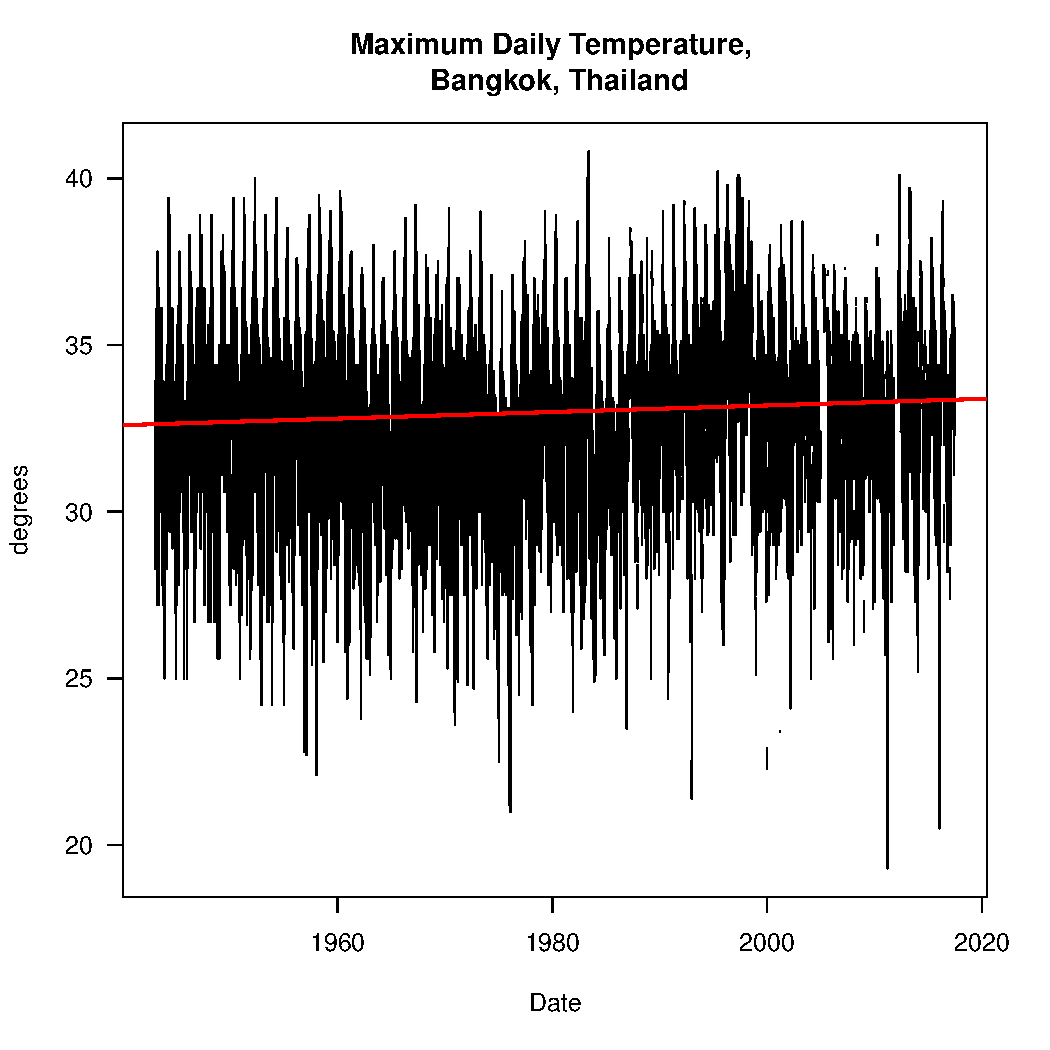
\includegraphics{Lab_Report_files/figure-latex/unnamed-chunk-5-1} \end{center}

\hypertarget{statistical-analysis}{%
\paragraph{Statistical Analysis}\label{statistical-analysis}}

As the unbagged data fell outside of normal distribution, a Paired
Samples Wilcoxon Test was used to evaluate the data. Using this test, a
p-value of 0.5839 was yielded. This p-value does not demonstrate
statistical significance, meaning that the null hypothesis may not be
rejected. A Two-Sample T-Test was also conducted, yielding a p-value of
0.2538. This also does not demonstrate statistical significance,
indicating that statistical significance likely would not be
demonstrated even if the data fell within normal distribution.

\hypertarget{discussion}{%
\subsubsection{Discussion}\label{discussion}}

\hypertarget{conclusion}{%
\subsubsection{Conclusion}\label{conclusion}}

\hypertarget{bibliography}{%
\subsubsection{Bibliography}\label{bibliography}}

Baalkhuyur F, Bin Dohaish E, Elhalwagy M, Alikunhi N, AlSuwailem A,
Røstad A, Coker D, Berumen M, Duarte C. 2018. Microplastic in the
gastrointestinal tract of fishes along the Saudi Arabian Red Sea coast.
Marine Pollution Bulletin. 107(A):407-415.~

Batel A, Linti F, Scherer M, Erdinger L, Braunbeck T. 2016. Transfer Of
Benzo{[}a{]}Pyrene From Microplastics To Artemia Nauplii And Further To
Zebrafish Via A Trophic Food Web Experiment: Cyp1a Induction And Visual
Tracking Of Persistent Organic Pollutants. Environmental Toxicology and
Chemistry. 35(7):1656-1666.~

Calafat A, Ye X, Wong L, Reidy J, Needham L. 2008. Exposure of the U.S.
Population to Bisphenol A and 4-tertiary-Octylphenol: 2003--2004.
Environmental Health Perspectives. 116(1):39-44.~

Fossi M, Marsili L, Baini M, Giannetti M, Coppola D, Guerranti C,
Caliani I, Minutoli R, Lauriano G, Finoia M, Rubegni F, Panigada S,
Berub M, Ramírez J, Panti C. 2016. Fin whales and microplastics: The
Mediterranean Sea and the Sea of Cortez scenarios. Environmental
Pollution. 209:68-78.~

{[}GESAMP{]} Joint Group of Experts on the Scientific Aspects of Marine
Environmental Protection. 2016. Sources, Fate And Effects Of
Microplastics In The Marine Environment: Part Two Of A Global
Assessment. GESAMP. 93:1-220.~

Karami A, Golieskardi A, Choo C, Larat V, Galloway T, Salamatinia B.
2017. The presence of microplastics in commercial salts from different
countries. 7:46173.~

Karbalaei S, Hanachi P, Walker T, Cole M. 2018. Occurrence, sources,
human health impacts and mitigation of microplastic pollution.
Environmental Science and Pollution Research. 25:36046-36063.~

Karlsson T, Vethaak A, Almrothd B, Ariese F, van Velzen M, Hassellöv M,
Leslie H. 2017. Screening for microplastics in sediment, water, marine
invertebrates and fish: Method development and microplastic
accumulation. Marine Pollution Bulletin. 122:403-408.~

Lachenmeier D, Kocareva J, Noack D, Kuballa T. 2015. Microplastic
identification in German beer -- an artefact of laboratory
contamination? Deutsche Lebensmittel-Rundschau. 111:437-440. ~

Loder M, Imhof H, Ladehoff M, Löschel L, Lorenz C, Mintenig S, Piehl S,
Primpke S, Schrank I, Laforsch C, Gerdts G. 2017. Enzymatic Purification
of Microplastics in Environmental Samples. Environmental Science and
Technology. 51:14283-14292.~

Maes T, Jessop R, Wellner N, Haupt K, Mayes A. 2017. A rapid-screening
approach to detect and quantify microplastics based on fluorescent
tagging with Nile Red. Scientific Reports. 7:44501.~

Quinn B, Murphy F, Ewins. 2017. Validation of density separation for the
rapid recovery of microplastics from sediment. Analytical Methods.
9(9):1491-1498.~

Rist S, Almroth B, Hartmann N, Karlsson T. 2018. A critical perspective
on early communications concerning human health aspects of
microplastics. Science of the Total Environment. 626:720-726.~

Rochman C, Tahir A, Williams S, Baxa D, Lam R, Miller J, Teh F,
Werorilangi S, Teh S. 2015. Anthropogenic debris in seafood: Plastic
debris and fibers from textiles in fish and bivalves sold for human
consumption. Scientific Reports. 5:14340.~

Wang W, Wang J. 2018. Investigation of microplastics in aquatic
environments: An overview of the methods used, from field sampling to
laboratory analysis. Trends in Analytical Chemistry. 108:195-202.~

de Witte B, Devriese L, Bekaert K, Hoffman S, Vandermeersch G, Cooreman
K, Robbens J. 2014. Quality assessment of the blue mussel (Mytilus
edulis): Comparison between commercial and wild types. Marine Pollution
Bulletin. 85:146-155. ~

Wright S, Kelly F. 2017. Plastic and Human Health: A Micro Issue?
Environmental Science and Technology. 51:6634-6647.~

\hypertarget{appendix-i-raw-data}{%
\subsubsection{Appendix I: Raw Data}\label{appendix-i-raw-data}}

\begin{table}[H]
\centering
\begin{tabular}{l|l|l|r|r|r|r|r|r}
\hline
X & Store & U.B....Bagged & Sample.. & Point.1 & Point.2 & Point.3 & Point.4 & Average\\
\hline
Cardenas U.B. \#1 & Cardenas & UB & 1 & 5 & 10 & 12 & 13 & 10.00\\
\hline
Cardenas U.B. \#2 & Cardenas & UB & 2 & 32 & 52 & 38 & 11 & 33.25\\
\hline
Cardenas B. \#1 & Cardenas & BG & 1 & 70 & 62 & 84 & 103 & 79.75\\
\hline
Cardenas B. \#2 & Cardenas & BG & 2 & 37 & 32 & 30 & 42 & 35.25\\
\hline
El Super U.B. \#1 & El Super & UB & 1 & 76 & 29 & 24 & 18 & 36.75\\
\hline
El Super U.B. \#2 & El Super & UB & 2 & 38 & 44 & 32 & 36 & 37.50\\
\hline
El Super B. \#1 & El Super & BG & 1 & 37 & 31 & 36 & 33 & 34.25\\
\hline
El Super B. \#2 & El Super & BG & 2 & 53 & 52 & 52 & 39 & 49.00\\
\hline
Sprouts U.B. \#1 & Sprouts & UB & 1 & 31 & 34 & 19 & 32 & 29.00\\
\hline
Sprouts U.B. \#2 & Sprouts & UB & 2 & 54 & 20 & 66 & 15 & 38.75\\
\hline
Sprouts B. \#1 & Sprouts & BG & 1 & 36 & 45 & 51 & 52 & 46.00\\
\hline
Sprouts B. \#2 & Sprouts & BG & 2 & 28 & 19 & 20 & 34 & 25.25\\
\hline
Stater Bros U.B. \#1 & Stater Bros & UB & 1 & 33 & 45 & 37 & 51 & 41.50\\
\hline
Stater Bros U.B. \#2 & Stater Bros & UB & 2 & 47 & 24 & 34 & 29 & 33.50\\
\hline
Stater Bros B. \#1 & Stater Bros & BG & 1 & 21 & 58 & 28 & 20 & 31.75\\
\hline
Stater Bros B. \#2 & Stater Bros & BG & 2 & 28 & 22 & 36 & 27 & 28.25\\
\hline
Super King U.B. \#1 & Super King & UB & 1 & 10 & 26 & 23 & 34 & 23.25\\
\hline
Super King U.B. \#2 & Super King & UB & 2 & 57 & 21 & 33 & 66 & 44.25\\
\hline
Super King B. \#1 & Super King & BG & 1 & 22 & 24 & 26 & 27 & 24.75\\
\hline
Super King B. \#2 & Super King & BG & 2 & 46 & 41 & 45 & 39 & 42.75\\
\hline
Blank \#1 & Blank & Blank & 1 & 18 & 10 & 55 & 31 & 28.50\\
\hline
Blank \#2 & Blank & Blank & 2 & 28 & 27 & 8 & 12 & 18.75\\
\hline
Blank \#3 & Blank & Blank & 3 & 24 & 46 & 25 & 13 & 27.00\\
\hline
\end{tabular}
\end{table}


\end{document}
